% Nallino, Part II p. 241: the prosthaphaeresis of longitude and its correction, redrawn from the print at the size of
% the print. The coordinates are those of a 400 dpi render of the figure (crop from x 386 pt, y 410 pt of the master
% page; y downward). The upper circle is the equant about E', the lower the deferent about M (marked with a dot);
% E is the Earth, H the centre of the epicycle on the deferent, h the point of the equant on the line E'H.
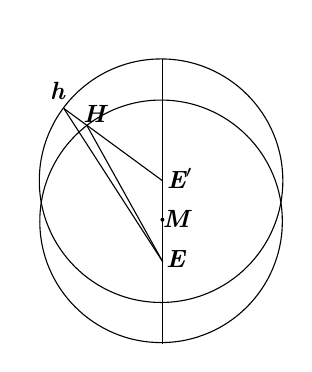
\begin{tikzpicture}[x=0.0635mm,y=-0.0635mm,line width=0.4pt,every node/.style={font=\bfseries\itshape\small,inner sep=1pt}]
\path (0,37);
\coordinate (Ep) at (269.5,343);
\coordinate (M) at (269.5,421);
\coordinate (E) at (270,505);
\coordinate (H) at (118,232);
\coordinate (h) at (72.2,198.4);
\draw (266.75,343) circle[radius=243.5];
\draw (266.75,424.25) circle[radius=242.5];
\draw (269.5,99) -- (269.5,669);
\draw (h) -- (Ep);
\draw (E) -- (h);
\draw (E) -- (H);
\fill (M) circle[radius=4];
\node at (59.5,164) {h};
\node at (133,210) {H};
\node at (297,338) {E\rlap{$'$}};
\node at (296.5,420) {M};
\node at (295.5,499.5) {E};
\end{tikzpicture}
